\documentclass{beamer}

\mode<presentation>
{
  %\usetheme{AnnArbor}
  \usetheme{Montpellier}
  %\usetheme{Hannover}
  %\usetheme{Singapore}
  %\usetheme{Madrid}
}

\newcommand*\oldmacro{}
\let\oldmacro\insertshorttitle% ursprüngliche Definition sichern
\renewcommand*\insertshorttitle{%
  \oldmacro
  \hfill\insertframenumber\,/\,\inserttotalframenumber}

\setbeamertemplate{navigation symbols}{}

\usepackage[english]{babel}

%\usepackage[latin1]{inputenc}
\usepackage[utf8]{inputenc}

%\usepackage{hyperref}

% WTF? times? serious?
%\usepackage{times}
\usepackage[T1]{fontenc}

\usepackage{listings}

%\usepackage{tabularx}

\title[Project Proposal]{Advanced Rendering \\ Project Proposal}

%\subtitle {Untertitel} (optional)

\author[Brauer, Heppner, Koza]
{S. Brauer \and S. Heppner \and A. Koza}

\institute[University of Paderborn]{Institute for Computer Science}

\date{\today}


\subject{Computer Science}

\pgfdeclareimage[height=0.5cm]{university-logo}{figures/upb_logo.png}
\logo{\pgfuseimage{university-logo}}



% Folgendes sollte gelöscht werden, wenn man nicht am Anfang jedes
% Unterabschnitts die Gliederung nochmal sehen möchte.
%\AtBeginSubsection[]
%{
%  \begin{frame}<beamer>{Gliederung}
%    \tableofcontents[currentsection,currentsubsection]
%  \end{frame}
%}



\begin{document}

\begin{frame}
  \titlepage
\end{frame}

\begin{frame}{Realistic Modelling}
\begin{minipage}[hbt]{0.45\textwidth}
	\begin{itemize}
		\item Model inner courtyard of university in detail
		\begin{itemize}
			\item Fountain
			\item Clock
			\item Vegetation
		\end{itemize}
	\end{itemize}	
\end{minipage}
\begin{minipage}[hbt]{0.45\textwidth}
	\begin{figure}
	\centering
	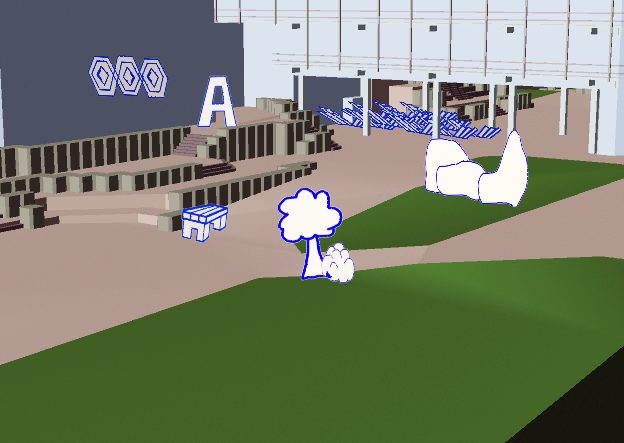
\includegraphics[width=4.5cm]{figures/models.png}
	\caption{Possible Model Arrangement}
	\end{figure}
\end{minipage}
\end{frame}

\begin{frame}{Image-Based Effects}
\begin{minipage}[hbt]{0.45\textwidth}
	\begin{itemize}
		\item "Mandatory" Effects: Skybox \& Normal Mapping
		\item Lens Flare, Blooming
		\item Screen Space Ambient Occlusion
	\end{itemize}	
\end{minipage}
\begin{minipage}[hbt]{0.45\textwidth}
	\begin{figure}
	\centering
	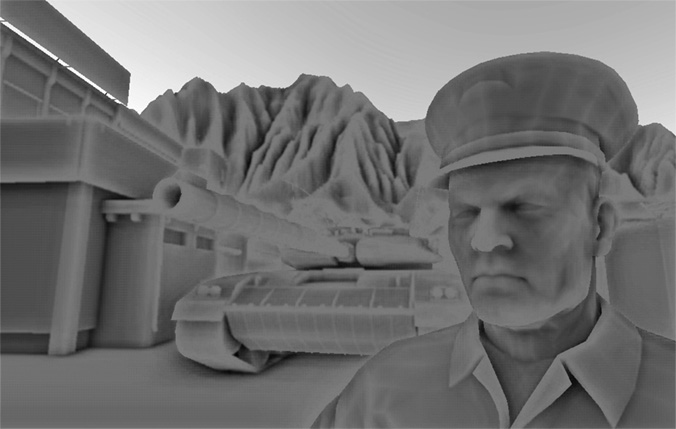
\includegraphics[width=4.5cm]{figures/ssao.jpg}
	\caption{SSAO}
	\end{figure}
\end{minipage}
\end{frame}

\begin{frame}{Change to Non-Photorealistic Rendering}
\begin{minipage}[hbt]{0.45\textwidth}
	\begin{itemize}
		\item Use a Cel-Shader as a contrast ...
		\item ... but at this point we don't want to spoiler too much
	\end{itemize}	
\end{minipage}
\begin{minipage}[hbt]{0.45\textwidth}
	\begin{figure}
	\centering
	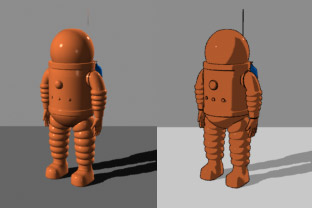
\includegraphics[width=4.5cm]{figures/toon_shader.jpg}
	\caption{Cel-(or Toon-)Shader}
	\end{figure}
\end{minipage}
\end{frame}


\end{document}
